% Created 2016-10-18 ti 11:39
\documentclass{article}
               \usepackage{listings}
\usepackage{color}
\usepackage{amsmath}
\usepackage{array}
\usepackage[T1]{fontenc}
\usepackage{natbib}
               \usepackage{authblk}
\newcommand{\EE}{\mathbb{E}}
\newcommand{\one}{1}
\newcommand{\VV}{\mathbb{V}}
\newcommand{\PP}{\mbox{P}}
\newcommand{\norm}{\mathcal{N}}
\newcommand{\lag}{N}
\newcommand{\str}{S}
\newcommand{\smin}{s^{\min}}
\newcommand{\smax}{s^{\max}}
\newcommand{\styp}{s^{*}}
\newcommand{\period}{[a,b]}
\newcommand{\periodK}{\ensuremath{[T_k,T_{k+1})}}
\newcommand{\K}{K}
\newcommand{\kk}{k}
\newcommand{\D}{D}
\newcommand{\B}{B}
\newcommand{\E}{E}
\newcommand{\XX}{X}
\newcommand{\LL}{L}
\newcommand{\QQ}{Q}
\newcommand{\Ru}{R}
\newcommand{\GG}{G}
\newcommand{\T}{T}
\newcommand{\st}{s}
\newcommand{\Nn}{N}
\newcommand{\A}{A}
\newcommand{\C}{C}
\newcommand{\uu}{u}
\newcommand{\vv}{v}
\newcommand{\zz}{z}
\newcommand{\ww}{w}
\newcommand{\M}{M}
\newcommand{\I}{I}
\newcommand{\RR}{R}

\lstset{
keywordstyle=\color{blue},
commentstyle=\color{red},stringstyle=\color[rgb]{0,.5,0},
literate={~}{$\sim$}{1},
basicstyle=\ttfamily\small,
columns=fullflexible,
breaklines=true,
breakatwhitespace=false,
numbers=left,
numberstyle=\ttfamily\tiny\color{gray},
stepnumber=1,
numbersep=10pt,
backgroundcolor=\color{white},
tabsize=4,
keepspaces=true,
showspaces=false,
showstringspaces=false,
xleftmargin=.23in,
frame=single,
basewidth={0.5em,0.4em},
}

\usepackage[utf8]{inputenc}
\usepackage[T1]{fontenc}
\usepackage{fixltx2e}
\usepackage{graphicx}
\usepackage{grffile}
\usepackage{longtable}
\usepackage{wrapfig}
\usepackage{rotating}
\usepackage[normalem]{ulem}
\usepackage{amsmath}
\usepackage{textcomp}
\usepackage{amssymb}
\usepackage{capt-of}
\usepackage{hyperref}
\author{Helene Charlotte Rytgaard and Thomas Alexander Gerds}
\date{\today}
\title{From \texttt{\%x\_recepter} to \texttt{Rcpp}: a new user interface and an efficient algorithm}
\hypersetup{
 pdfauthor={Helene Charlotte Rytgaard and Thomas Alexander Gerds},
 pdftitle={From \texttt{\%x\_recepter} to \texttt{Rcpp}: a new user interface and an efficient algorithm},
 pdfkeywords={},
 pdfsubject={},
 pdfcreator={Emacs 25.1.1 (Org mode 8.3.6)}, 
 pdflang={English}}
\begin{document}

\maketitle
\section{Introduction}
\label{sec:orgheadline1}

The Danish National Prescription Registry (NCBI) provides
individual-level data on all prescription drugs sold in Danish
community pharmacies since 1994 \citep{kildemoes2011danish}. Effects and
side effects of drugs can be assessed in a Danish nation wide registry
studies. For this the prescription data are linked to the cause of
death register and other Danish registries
\citep{thygesen2011introduction}.

This document describes a complex algorithm for the computation of
drug exposure strength and length relative to a prespecified study
period \period. Note that the start of the study period has to be
after the start of the registry.

\section{Drug prescription data}
\label{sec:orgheadline2}

We describe the data of a single person who has purchased the drug of
interest at \({K}\) different dates in the study period \period. The
setup can easily be generalized to multiple individuals. The set of
ordered drug purchase dates for one individual is denoted as
\begin{equation*}
{T}_1< \cdots< {T}_{K}.
\end{equation*}
One package of each drug product is defined by the drug strength
\(\str\) of the smallest unit (e.g., one pill or half a pill) and the
amount of such units that it contains. For each drug we distinguish
\(J\ge 1\) different package types according to the different
strengths: \(\str_1,\dots,\str_J\). For each drug strength \(\str_j\) the values \(\smin_j\), \(\smax_j\), \(\styp_j\)
 define the minimal, maximal and typical dose per day, respectively. Note that
the original SAS macro allowed at most 4 different package types. We
combine all packages purchased on the same date that have the same
strength. The number of smallest units, \(\smin_j\), of type
\(j\) purchased on date \(T_k\) is denoted by \(\tilde{n}_{jk}\). Thus, the
total amount \(D_k\) of the drug purchased on date \(T_k\) is given by
the formula
\begin{align*}
D_k=\frac{1}{\# J_k} \sum_{j=1}^J\tilde{n}_{jk}\smin_{j} = \sum_{j=1}^J n_{jk} \smin_j,
\end{align*}
where \(\# J_k = \sum_{j=1} ^J \one \lbrace n_{jk}>0\rbrace\) is the number of different drugs purchased on date \(T_k\). Note that \(n_{jk} = \tilde{n}_{jk} \mathbin{/} (\# J_k)\). \\
FIXME: does it actually  make sense to divide with number of different drugs (as done in macro)?\\
FIXME: this way of defining the dosis does not fit with the calculation of dosis sequences\ldots{} 
Figure \ref{fig:1} illustrates the data

\begin{figure}[htb]
\centering
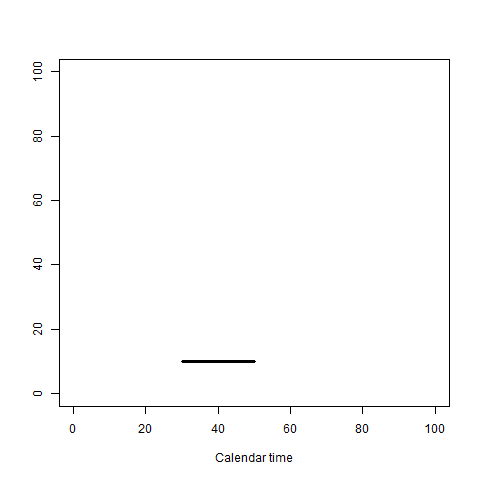
\includegraphics[width=0.7\textwidth]{./drug-data.png}
\caption{\label{fig:1}
label til figure}
\end{figure}

\section{Hospital admission data}
\label{sec:orgheadline3}

Hospitals usually deliver drugs for their patients. It is therefore
hensigtsmaessig to take into account periods of hospitalization in the
calculation of exposure lengths. For a single individual we define up
to \(Q\) periods of hospitalization by the admission dates
\({L}_1,\ldots, {L}_{{Q}}\) and the corresponding discharge dates
\({R}_1,\ldots, {R}_{{Q}}\). 

We compute the number of days hospitalized in the period \(\periodK\)
as:
\begin{align*} 
{A}_{k} &= \sum_{q=1}^{{Q}} \max \big( 0,\,\min \left({T}_{k+1},{R}_{q}\right) - \max\left({T}_{k}, {L}_{q}\right)
\big).
\intertext{Accordingly the number of non-hospitalized days in \(\periodK\) is:}
C_k &= \left({T}_{k+1} - {T}_{k}\right) - {A}_{k}.
\end{align*}

FIXME: 
\begin{itemize}
\item need to limit to the study period \period?
\item is the day \(T_{k+1}\) included in \periodK or not?\}[3cm]
\end{itemize}

\section{Exposure strength and exposure lengths}
\label{sec:orgheadline7}

The aim is to calculate the ends of the exposure periods \(E_k\) and
for each exposure period the exposure strength per day \(X_k\). The
calculations of exposure are based on the drug prescription data and
the hospitalization dates and depend further on the following
parameters. An integer \(\lag\) defines the number of
prescription dates back in time to use in the calculations of exposure
in a given period \periodK.

To express the exposure in period \(\periodK\) we first note that
based on the total drug purchase on date \(T_k\) the individual can be
exposed at most \(n_k=\sum_{j=1}^J n_{jk}\) days. 

FIXME: would it not be more logical to use \(\tilde n_k = n_{jk}
\frac{S_j}{\smin_j}\) instead of \(n_k\)? Helene: Not relevant any longer.


We use the following notation to indicate if the maximal number of
exposure days exceeds the non-hospitalized days in period \periodK:
\begin{align*} 
u_{k} = \begin{cases}
0, & n_{k} \le C_k\\
1, & n_{k} > C_k
\end{cases}.
\end{align*}
We use \(\bar{Y}_{k}\) to denote the history of a variable \(Y\) up to
period \(k\). For example,
\begin{align*}
\bar{D}_{k} = \left( D_{k} ,D_{k-1}, \ldots, D_1\right)
\end{align*}
is the history of total drug purchase until and including date \(T_k\).

\subsubsection{Calculating the doses, \({X}_1, \ldots, {X}_{{K}}\)}
\label{sec:orgheadline4}

HELENE: we need to adapt the following formula to the new notations.

\begin{align*} 
&{X}_{k} = (1-u_k)\, (1-u_{k-1}) \, d_{k}^*
\\ & \qquad + \, u_{k-1}\, \Big(1\{D_{k-1}=D_{k}\} \, {z}(
\bar{S}_{k}, \bar{D}_{k}, \bar{{C}}_{k} ) + 1\{D_{k-1}\ne D_{k}\}\,
{w}( \bar{S}_{k}, \bar{D}_{k}, \bar{{C}}_{k} ) \Big) \\ & \qquad +
\,u_{k} \,(1-u_{k-1})\, {w}( \bar{S}_{k}, \bar{D}_{k},
\bar{{C}}_{k} ).
\end{align*}

Here, ${z}( \bar{S}_{k}, \bar{D}_{k}, \bar{{C}}_{k} )$ and
${w}( \bar{S}_{k}, \bar{D}_{k}, \bar{{C}}_{k} )$ are
calculated from the mean dose 
\begin{align*}
M^{{z}, {w}}_{jk} = \frac{\sum_{i \in {I}^{z, w}_{k}}n_{ij}\smin_j}{\sum_{i \in {I}^{{z}, {w}}_{k}} {C}_i},
\end{align*}
where

\begin{align*}
{I}^{{w}}_{k} = \big\lbrace \min \lbrace i : u_i = \cdots = u_{k-1} =1 \rbrace, \ldots, k-1\big\rbrace,
\end{align*}
and, 
\begin{align*}
{I}^{{z}}_{k} = \big\lbrace \max \big( &\min \lbrace i : u_i = \cdots = u_{k-1} =1 \rbrace, \\
&  \min \lbrace i : g( s_i) = \cdots =g( s_{k})  \rbrace \big), \ldots, k-1 \big\rbrace,
\end{align*}
where 
\begin{align*}
s_i = \frac{1}{\# J_i}  \sum_{j=1}^J \one \lbrace n_{ij} > 0\rbrace\, \str_{j}, \quad \text{and} \quad g(x) = \sum_{j=1}^{J-1} \one \lbrace S_{j} \le x<  S_{j+1} \rbrace\, S_{j}, 
\end{align*}
according to
 \begin{align*}
{z}( \bar{S}_{k}, \bar{D}_{k}, \bar{{C}}_{k} )& = \sum_{j=1}^J \text{round}\,\Big ( M_{jk}^{{z}} \mathbin{/} \smin_{j}\Big) \cdot \smin_{j}, \\
{w}( \bar{S}_{k}, \bar{D}_{k}, \bar{{C}}_{k} )& = \frac{1}{\#J_k}\sum_{j=1}^J\max \Big(\one \lbrace n_{jk} >0\rbrace \, \smin_j, \, \one \lbrace M_{jk}^{{w}} > \smax_{j} \rbrace\, \smax_{j} + \one\lbrace M_{jk}^{{w}} < \smin_{j} \rbrace\, 
 \smin_{j}\\
& + \one \lbrace \smin_{j} \le M_{jk}^{{w}} \le \smax_{j} \rbrace \,\styp_{j}\Big),
\end{align*}

where, again, \(\#J_k= \sum_{j= 1}^J \one\lbrace n_{jk} > 0\rbrace\) is the number of different drugs purchased on date \(T_k\).\\


\subsubsection{Calculating the end dates, \({E}_1,\ldots, {E}_{k}\)}
\label{sec:orgheadline5}

\begin{align*}
{E}_{k}= \min \bigg[ {T}_{k+1}-1, \, (1-u_{k})\, (1-u_{k-1})  \, \bigg( {T}_{k} - 1+ \text{round} \left( \tfrac{D_{k} + {R}_{k}}{d_{k}^*} \right)\bigg) + \\
 \left(1-(1-u_{k})\, (1-u_{k-1}) \right)  \, \bigg( {T}_{k} - 1+ \text{round} \left( \tfrac{D_{k} + {R}_{k}}{{X}_{k}} \right)\bigg)\bigg]
\end{align*}

\subsubsection{Calculating the leftover dose, \({R}_1,\ldots, {R}_{k}\)}
\label{sec:orgheadline6}

\begin{align*}
{R}_{k} = \Big( D_{k-1} + {R}_{k-1} - {X}_{k-1} \left( {E}_{k-1} - {T}_{k-1} \right) \Big) \, u_{k}.\end{align*}



\section{User interface}
\label{sec:orgheadline9}

\subsection{Output}
\label{sec:orgheadline8}

The output consists of:

\begin{itemize}
\item \({B}_1, \ldots, B_{{K}}\): Starting dates for each prescription
period.
\item \({E}_1, \ldots, E_{{K}}\): End dates for each prescription period.
\item \({X}_1, \ldots, {X}_{{K}}\): Calculated dose for each prescription
period.
\end{itemize}

\bibliographystyle{chicago}
\bibliography{heaven}
\end{document}